\documentclass[a2,landscape]{a0poster}
\usepackage{mathptmx}
\usepackage[scaled=.90]{helvet}
\usepackage{courier}
\usepackage{postercols}
\usepackage{flowfram}
\usepackage{graphicx}
\usepackage{adjustbox}
\usepackage{tikz}

\setlength{\vcolumnsep}{\baselineskip}
\setlength{\columnsep}{\vcolumnsep}
\Ncolumntop{static}{3}{1.75in}
\setstaticframe{1}{label={title}}
\newlength\offset
\setlength{\offset}{5in}
\addtolength{\offset}{\vcolumnsep}

%\computeflowframearea{2,3}
%\addtolength{\ffareaheight}{-\offset}
%\setflowframe{2,3}{y=\offset,height=\ffareaheight}
%\newstaticframe{\ffareawidth}{5in}{\ffareax}{0in}[table]

\newcommand{\redborder}[1]{\tikz \node[draw,rectangle,blue] {#1};}

\setstaticframe{2}{clear}
\setallflowframes{border=plain, bordercolor=blue}
\setallstaticframes{border=plain, bordercolor=blue}
\setallflowframes{border=redborder}
\title{Locy: Energy-efficient sensing with Android smartphones.}
\author{Martin Kukla (Supervisor: Dr Tristan Henderson)}
\date{}
\begin{document}
\begin{staticcontents*}{title}
\maketitle	 
\end{staticcontents*}
\thispagestyle{empty}

\setlength{\tabcolsep}{3pt}


\begin{center}
\section*{Introduction}
\end{center}
		
\begin{itemize}
   \item Phone sensing may be utilized by mobile applications to provide \textbf{advanced services} such as navigation systems.
   
\begin{center}
	
\includegraphics[scale=0.08]{plots/logo_yelp}   
	
\includegraphics[scale=0.35]{plots/logo_apple_maps}
   
\includegraphics[scale=0.08]{plots/logo_google_maps}
	
\includegraphics[scale=0.3]{plots/logo_facebook}
	
\includegraphics[scale=0.4]{plots/logo_mhealth}\\
	
\includegraphics[scale=0.4]{plots/logo_foursquare}
	
\includegraphics[scale=1.2]{plots/logo_google_now}
\end{center}
	
   \item \textbf{Phone sensing} fetches raw sensor data\ (e.g. from an accelerometer) and tries to extract high-level information from it\ (e.g. a user is walking).
   \item Phone sensing has \textbf{high energy demands}, which is crucially important to mobile phone users.
   \item To solve the problem:
	   \begin{itemize}
   			\item investigate three different devices.
   			\item establish the energy efficiency of their sensors.
   			\item leverage results for energy-efficient sensing.
   			\item build \textbf{Locy}, an energy efficient sensing library.
   			\item evaluate its energy efficiency in real-life scenarios.
	   \end{itemize}
  \end{itemize}
  
\vspace{0.9cm}
\begin{center}

\includegraphics[scale=0.7]{plots/low_battery}

\includegraphics[scale=0.7]{plots/sad_face}
\end{center}

\mbox{}\framebreak
\begin{center}
\section*{Solution}
\end{center}
\begin{itemize}
   \item Energy efficiency of sensors are \textbf{different among the three devices}.\\
   \includegraphics[width=16cm, height=7.5cm]{plots/shared}

 \begin{tabular}[t]{p{8.0cm} p{9.0cm}}
       \vspace{0cm} However, \textbf{accelerometer is always more energy-efficient} than the standard localization sensors. & \vspace{0cm}\includegraphics[scale=0.6]{plots/acc_vs_loc}
      \end{tabular}

   \item \textbf{Locy} leverages an efficient \textbf{accelerometer}:
  	   \begin{itemize}		
  	   \item if a user is not moving, it \textbf{switches off GPS}. 
  	   \item \textbf{movement detection} based on "peaks"\ (steps):
  	   %based on the standard deviation of the total magnitude over accelerometer data).\\
  	   
  	   \hspace{0.75cm}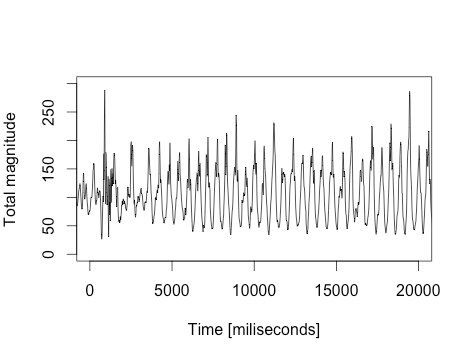
\includegraphics[scale=0.4]{plots/walking}
	   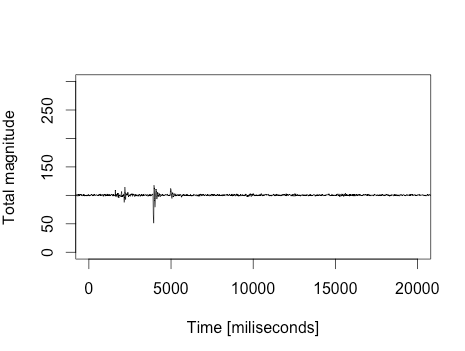
\includegraphics[scale=0.4]{plots/no_walking}
  	   \item Locy uses \textbf{duty-cycling sampling}\ (sleeping periods interleaves sampling), whose ratio\ (sampling over sleeping period) is \textbf{adaptive according to current battery life}. 
    \end{itemize} 
  \end{itemize}


\mbox{}\framebreak
\begin{center}
\section*{Evaluation}
\end{center}
\begin{itemize}
   \item \textbf{scenario one}:

\begin{tabular}[t]{p{8.0cm} p{8.0cm}}
       \vspace{0cm}\includegraphics[scale=0.65]{plots/locy_eval_inplace} &  \vspace{0cm}While a user is staying in one place, Locy is more energy-efficient than the naive GPS localization.
      \end{tabular}
\vspace{0.3cm}
   \item \textbf{scenario two}:

\begin{tabular}[t]{p{8.0cm} p{8.0cm}}
	\vspace{0cm}\includegraphics[scale=0.65]{plots/locy_eval_other} &  \vspace{0cm}While a user is half of the time moving and the rest of the time he is staying in one place, Locy is more energy-efficient than the naive GPS localization.
\end{tabular}
  \end{itemize}

\begin{center}
\section*{Conclusions}
\end{center}

\textbf{Locy} is more energy-efficient than the standard Android implementation. 
\vspace{1.25cm}
\begin{center}

\includegraphics[scale=0.7]{plots/full_battery}

\includegraphics[scale=0.7]{plots/happy_face}
\end{center}


\end{document}
